
\documentclass[12pt]{article}
 
\usepackage[margin=1in]{geometry} 
\usepackage{multicol,caption}
\usepackage{graphicx}
\usepackage{multicol}
\usepackage{lipsum}
\usepackage{float}
\usepackage{graphics}
\usepackage[utf8x]{inputenc}
\usepackage{amsmath}
\usepackage{listings}
\usepackage{amssymb}

\newcommand{\N}{\mathbb{N}}
\newcommand{\Z}{\mathbb{Z}}
\newcommand{\R}{\mathbb{R}}
 \newenvironment{Figure}
  {\par\medskip\noindent\minipage{\linewidth}}
  {\endminipage\par\medskip}

\begin{document}

 
\title{Progetto Sistemi Intelligenti - Alberto Borghese
Riconoscitore di cifre manoscritte}%replace X with the appropriate number
\author{Francesco Bertolotti} %if necessary, replace with your course title

\maketitle
\newpage
\tableofcontents
\newpage

\section{Introduction}
Come concordato, ho deciso di sfruttare alcuni concetti mostrati
durante il corso per implementare un riconoscitore di cifre manoscritte 
sfruttando le reti neurali. Il progetto è stato svolto in python utilizzando diverse librerie.
E' stato utilizzato il dataset del MNIST.\\

%%%%%%%%%%%%%%%%%%%%%%%%%%%%%%%%%%%%%%%%%%%%%%%%%%%%%%%%%%%%%%%%%%%%%%%%%%%
%%%%%%%%%%%%%%%%%%%%%%%%%%%%%%%%%%%%%%%%%%%%%%%%%%%%%%%%%%%%%%%%%%%%%%%%%%%
%%%%%%%%%%%%%%%%%%%%%%%%%%%%%%%%%%%%%%%%%%%%%%%%%%%%%%%%%%%%%%%%%%%%%%%%%%%

\subsection{Scripts}
Sono stati prodotti quattro script in python: 
\begin{enumerate}
    \item dataset.py: Legge e carica il dataset mnist applicando eventualmente
                      un balancing delle diverse classi.
    \item trainer.py: Sfrutta i dati caricati da dataset.py per andare
                      ad addestrare una rete neurale. Alla fine del training
                      salva il modello migliore e le immagini relative alla
                      storia della loss e della accuracy durante la fase di training.
    \item models.py: E' una semplice classe contenente alcune tipologie di modello
                     neurale utilizzate da trainer.py.
    \item recognizer.py: Carica uno dei modelli salvati, apre una finestra
                         e ad ogni cifra disegnata scrive da terminale la confidenza
                         con cui ogni cifra viene riconosciuta. 
\end{enumerate}

%%%%%%%%%%%%%%%%%%%%%%%%%%%%%%%%%%%%%%%%%%%%%%%%%%%%%%%%%%%%%%%%%%%%%%%%%%%
%%%%%%%%%%%%%%%%%%%%%%%%%%%%%%%%%%%%%%%%%%%%%%%%%%%%%%%%%%%%%%%%%%%%%%%%%%%
%%%%%%%%%%%%%%%%%%%%%%%%%%%%%%%%%%%%%%%%%%%%%%%%%%%%%%%%%%%%%%%%%%%%%%%%%%%

\subsection{Dependency}
Le librerie utilizzate in python sono elencate di seguito:
\begin{enumerate}
    \item Keras\cite{keras}: Una nota API ad alto livello per reti neurali.
    \item numpy: Un pacchetto per il calcolo scientifico.
    \item optparse: Un pacchetto per la gestione di opzioni CLI.
    \item tensorflow\cite{tensorflow}: engine backend per keras, capace di sfruttare anche le GPU.
    \item opencv\cite{opencv}: API per la gestione di immagini.
\end{enumerate}

%%%%%%%%%%%%%%%%%%%%%%%%%%%%%%%%%%%%%%%%%%%%%%%%%%%%%%%%%%%%%%%%%%%%%%%%%%%
%%%%%%%%%%%%%%%%%%%%%%%%%%%%%%%%%%%%%%%%%%%%%%%%%%%%%%%%%%%%%%%%%%%%%%%%%%%
%%%%%%%%%%%%%%%%%%%%%%%%%%%%%%%%%%%%%%%%%%%%%%%%%%%%%%%%%%%%%%%%%%%%%%%%%%%

\subsection{Parameters}
Per quanto riguarda trainer.py:
\begin{enumerate}
    \item "-d", "--directory": permette di scegliere una cartella di destinazione
    per il salvataggio del modello.
    \item "-s", "--batch": permette di scegliere la dimensione del batch con cui
    effettuare l'addestramento.
    \item "-e", "--epochs": permette di scegliere il numero di epoche per
    cui si vuole fare l'addestramento.
    \item "-b", "--balance": permette di specificare se si vuole effettuare
    un bilanciamento delle diversi classi prima di cominciare l'addestramento.
    \item "-c", "--committee": permette di selezionare il numero di reti che si 
    vogliono addestrare, con lo scopo di generare una pool di esperti che prenderà
    le decisioni per maggioranza.
    \item "-m", "--modelname": permette di scegliere il tipo del modello, questi
    sono descritti nel file "models.py".
\end{enumerate}
Ad ogni addestramento verrano generati i seguenti file:

\begin{enumerate}
    \item "test\_loss\_acc.png", "train\_loss\_acc.png": sono il plot dell'accuratezza e della loss
    rispetto al training set e al test set generato epoca per epoca.
    \item "model.png": l'immagine rappresentante il modello.
    \item "model0.best.hdf5": il migliore modello addestrato in termini di accuratezza e loss.
\end{enumerate}

Esempi di esecuzioni:

\begin{lstlisting}
    python3 trainer.py -s 512 -m "MLPNN_type0" -e 100 -c 20 -b
    python3 trainer.py -s 128 -m "CNN2D_type0" -e 20 -c 10 -b
    python3 trainer.py -s 512 -m "MLPNN_type0" -e 100 -c 20
    python3 trainer.py -s 128 -m "CNN2D_type0" -e 20 -c 10
    python3 trainer.py -s 512 -m "MLPNN_type0" -e 100
    python3 trainer.py -s 128 -m "CNN2D_type0" -e 20
    python3 trainer.py
\end{lstlisting}

Per quanto riguarda recognizer.py:

\begin{enumerate}
    \item "-f", "--modeldir": permette di indicare la directory in cui un modello
    è stato salvato.
    \item "-v", "--verbose": in caso sia presente, oltre a stampare la confidenze
    di riconoscimento per ogni cifra, stampa anche la griglia $28\times28$ utilizzata per il riconoscimento.

\end{enumerate}

Esempi di esecuzioni:

\begin{lstlisting}
    python3 recognizer.py -f ./mnist_models/MLPNN_type0-batch512-balanced-committee20/ -v    
    python3 recognizer.py -f ./mnist_models/MLPNN_type0-batch512-balanced-committee20/    
    python3 recognizer.py    
\end{lstlisting}

\newpage

%%%%%%%%%%%%%%%%%%%%%%%%%%%%%%%%%%%%%%%%%%%%%%%%%%%%%%%%%%%%%%%%%%%%%%%%%%%
%%%%%%%%%%%%%%%%%%%%%%%%%%%%%%%%%%%%%%%%%%%%%%%%%%%%%%%%%%%%%%%%%%%%%%%%%%%
%%%%%%%%%%%%%%%%%%%%%%%%%%%%%%%%%%%%%%%%%%%%%%%%%%%%%%%%%%%%%%%%%%%%%%%%%%%

\section{Background}

Alcune generalità preliminari sulle nozioni utilizzate
per implementare il progetto.

%%%%%%%%%%%%%%%%%%%%%%%%%%%%%%%%%%%%%%%%%%%%%%%%%%%%%%%%%%%%%%%%%%%%%%%%%%%
%%%%%%%%%%%%%%%%%%%%%%%%%%%%%%%%%%%%%%%%%%%%%%%%%%%%%%%%%%%%%%%%%%%%%%%%%%%
%%%%%%%%%%%%%%%%%%%%%%%%%%%%%%%%%%%%%%%%%%%%%%%%%%%%%%%%%%%%%%%%%%%%%%%%%%%

\subsection{Gradient descent}

La discesa del gradiente è un metodo di ottimizzazione
per trovare un minimo assoluto o locale di una funzione.\\

L'idea su cui questa tecnica è basata è estremamente semplice.\\
Andiamo inizialmente a scegliere dei valori iniziali per i parametri (anche casuali)
della funzione obbiettivo (differenziabile). A questo punto calcoliamo 
la derivata rispetto ai singoli parametri, 
troviamo quindi il gradiente. Aggiorniamo i parametri in accordo con il gradiente.\\

Notaiamo che il gradiente rappresenta un vettore in uno spazio 
multidimensionale e ci da la direzione lungo il quale l'ipercurva cresce.
Se volessimo trovare un minimo anzichè un massimo sarebbe sufficiente
seguirne il negativo.\\

\begin{figure}[H]{}
    \centering
    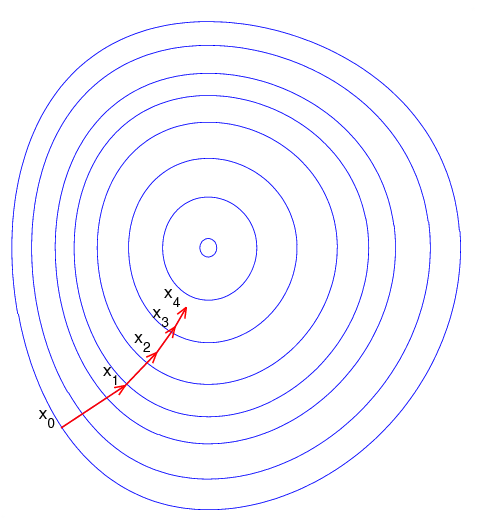
\includegraphics[scale=0.5]{../images/grd.png}
    \captionof{figure}{Discesa del gradiente}\label{fig:cc}
\end{figure}

Per chiarire meglio il metodo facciamo un esempio con la seguente funzione:

\begin{equation}f(x)=4x^3-9x^2\end{equation}
\begin{figure}[H]{}
    \centering
    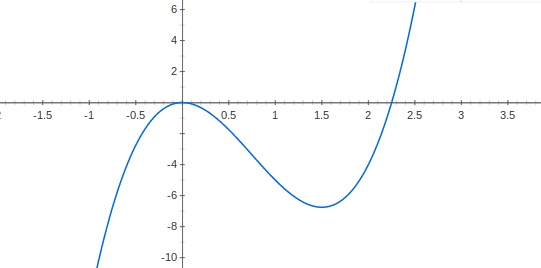
\includegraphics[scale=0.5]{../images/e.png}
    \captionof{figure}{funzione esempio}\label{fig:cc}
\end{figure}

La derivata invece è: $f(x)=12x^2-18x$.\\
A questo punto iteriamo il procedimento:\\


\begin{lstlisting}
inizializza i parametri;
iterazione = 0;
while iterazione < soglia:
    iterazione += 1;
    calcola gradiente;
    aggiorna parametri;
\end{lstlisting}


Seguiamo l'algoritmo per alcuni step applicando un fattore
moltiplicativo di 0.01; partiamo con $x=2.5$:

\begin{equation}f(2.5)=6.25\end{equation}
\begin{equation}f'(2.5)=30\end{equation}

Dovremmo spostarci di 30, quindi -0.3.

\begin{equation}f(2.2)=-0.96\end{equation}
\begin{equation}f'(2.2)=18.48\end{equation}

Adesso di -0.1.

\begin{equation}f(2.1)=-0.2.646\end{equation}
\begin{equation}f'(2.1)=15.12\end{equation}

Ancora di -0.1.

\begin{equation}f(2)=-4\end{equation}
\begin{equation}f'(2)=12\end{equation}

$\dots$\\

In ultimo chiariamo l'importanza del fattore moltiplicativo,
chiamato in seguito "learning rate". Un fattore eccessivamente grande 
porta a delle modifiche (salti) altrettanto grandi quindi si ha il rischio
di avere delle discese inutilmente lente in alcuni casi.
Mentre un fattore piccolo necessità di più tempo per trovare
un minimo già solo per il motivo che si compiono "salti ridotti".

\begin{figure}[H]{}
    \centering
    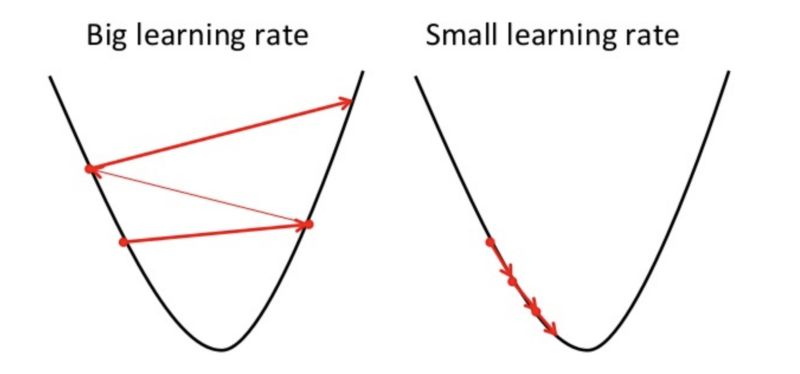
\includegraphics[scale=0.5]{../images/lr.png}
    \captionof{figure}{esempio di discesa del gradiente
    nel caso di un fattore moltiplicatico grande e piccolo.}\label{fig:cc}
\end{figure}


%%%%%%%%%%%%%%%%%%%%%%%%%%%%%%%%%%%%%%%%%%%%%%%%%%%%%%%%%%%%%%%%%%%%%%%%%%%
%%%%%%%%%%%%%%%%%%%%%%%%%%%%%%%%%%%%%%%%%%%%%%%%%%%%%%%%%%%%%%%%%%%%%%%%%%%
%%%%%%%%%%%%%%%%%%%%%%%%%%%%%%%%%%%%%%%%%%%%%%%%%%%%%%%%%%%%%%%%%%%%%%%%%%%

\subsection{MLPNN: Multi Layer Perceptron Neural Network}

Un Multi Layer Perceptron è un specifico tipo di rete neurale di
tipo feedforward. Un MLP è costituido da almeno 3 layer di
neuroni, ognuno dei quali completamente connesso a tutti i neuroni
dei livelli precedenti e successivi.
Ogni neurone prende come input gli output dei neuroni dei layer
precedenti, ne fa la somma pesata e applica una funzione di attivazione.

\begin{figure}[H]{}
    \centering
    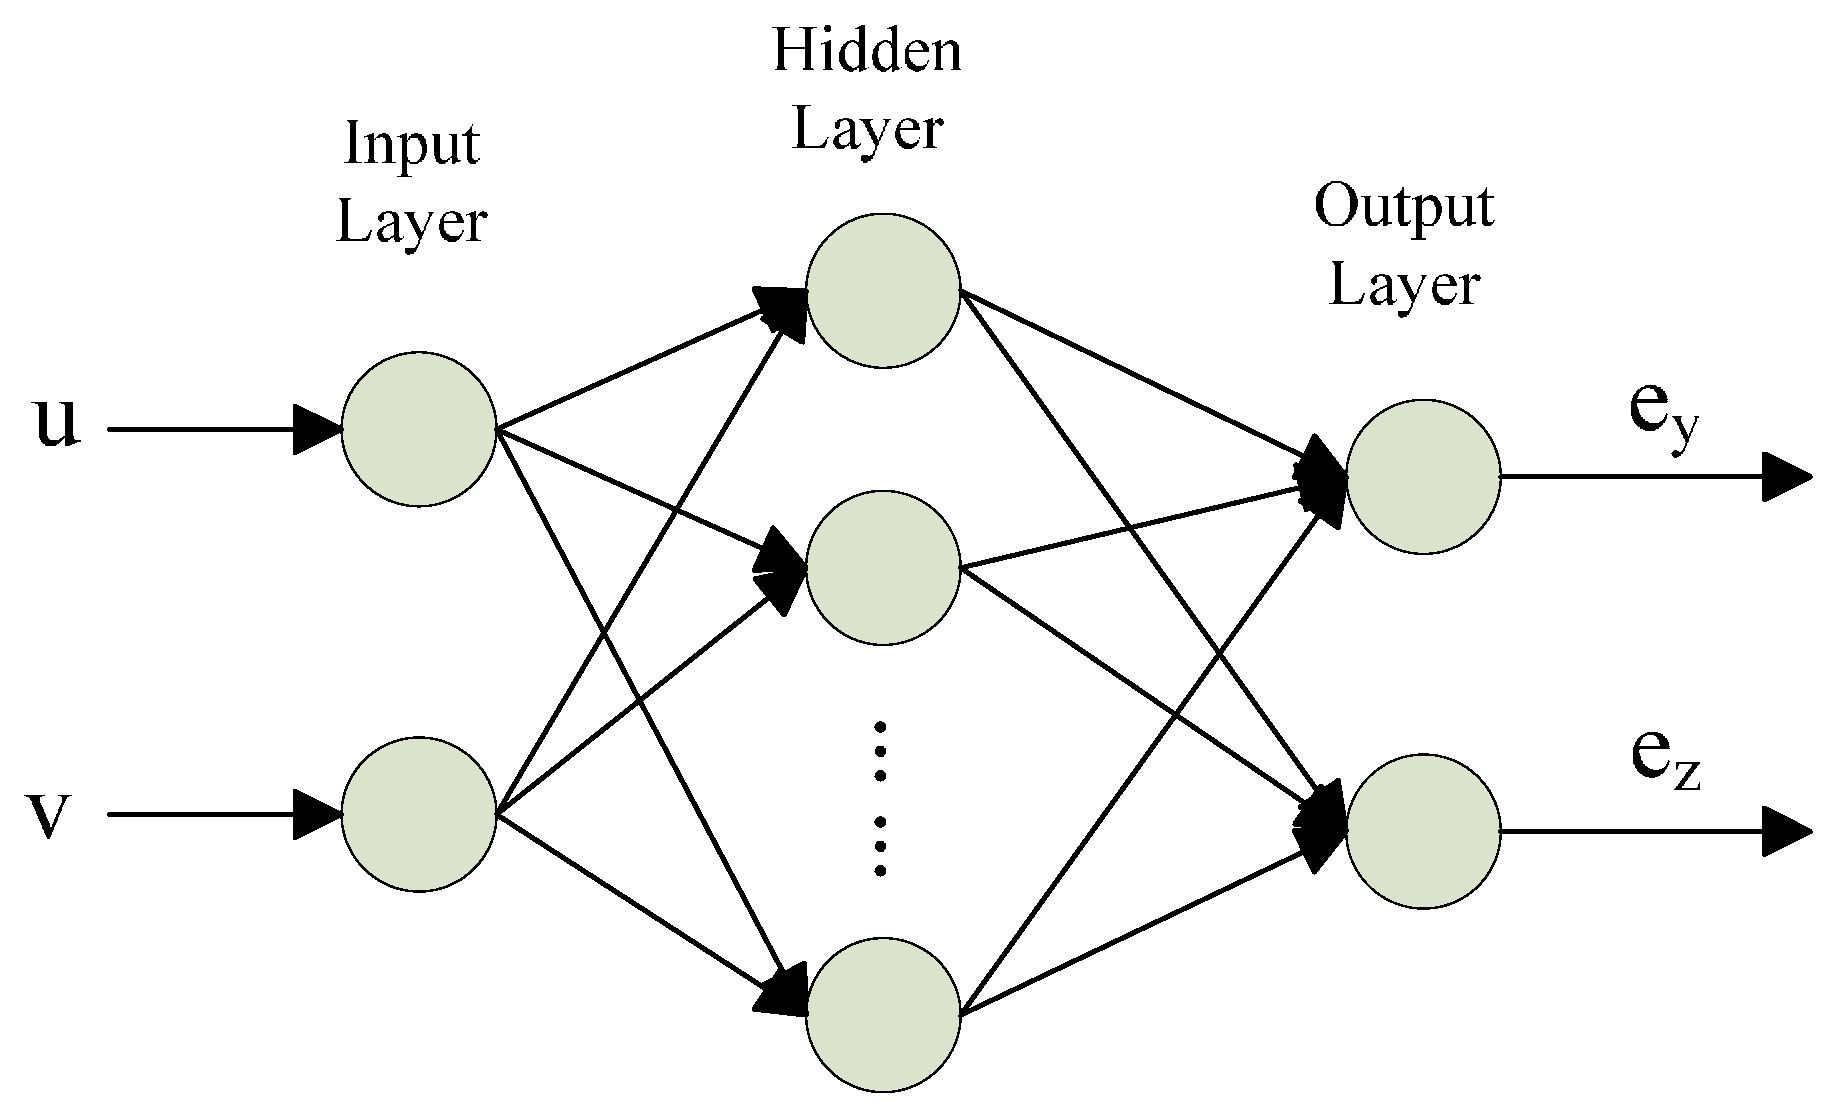
\includegraphics[scale=0.8]{../images/mlpnn.png}
    \captionof{figure}{esempio di MLPNN}\label{fig:cc}
\end{figure}

Il primo layer viene solitamente definito di input, mentre
l'ultimo prende il nome di "layer di output", a tutti gli
altri ci si riferisci come "hidden layers".\\

Un MLPNN è solitamente utilizzato in abito di classificazione,
o regressione.\\

L'addestramento di questa rete, in ambito supervisionato, avviene 
minimizzando la Loss function. L'idea è quella di andare
ridurre l'errore che la rete commette rispetto a quello che vorremmo.
Una loss function comunemente usata è la seguente:

\begin{equation}
\frac{1}{n}\sum_{i=1}^{n} \frac{1}{2}(t_i-o_i)^2 
\end{equation}
Dove:
\begin{enumerate}
    \item $n$ è il numero di casi nel dataset.
    \item $t_i$ è il risultato che vorremmo ottenere, in classificazione, la classe target.
    \item $o_i$ è l'output della rete.
\end{enumerate}

Ottenere una soluzione esatta dalla loss function è possibile
solamente per casi banali. In generale siamo costretti 
a cercare delle soluzioni approssimate, queste vengono ottenuto
attraverso la minimizzazione del gradiente.\\

Per completezza diamo la formula per ottenere il gradiente:

\begin{equation}
\frac{\delta E}{\delta o_j} = \delta_j o_j
\end{equation}

Dove:

\begin{equation}
    \delta_j = \frac{\delta E}{\delta o_j}\frac{\delta o_j}{\delta net_j} = 
    \begin{cases} 
        (o_j - t_j)\sigma'(z_j)\text{  se il neurone è di output}\\
        (\sum_{l \in L} w_jl\delta_l)\sigma'(z_j)\text{  se il neurone è interno}
    \end{cases}
\end{equation}

Dove:

\begin{enumerate}
    \item $L$ rappresenta l'insieme di neuroni di un determinato layer.
    \item $w_{ij}$ è il peso che va dall' i-esimo neuroe del layer $L-1$ al
    j-esimo neurone del layer $L$.
    \item $z_j$ è l'output non attivato del j-esimo neurone del layer $L-1$.
    \item $\sigma$ è la funzione di attivazione scelta.
\end{enumerate}

L'aggiornamento di ciascun peso quindi prende la seguente forma:

\begin{equation}
w_{ij} = w_{ij} - \alpha\Delta w_{ij}
\end{equation}

Dove $\alpha$ rappresenta il learning rate da applicare,
solitamente è un numero basso compreso tra 0 e 1.
Lo scopo di $\alpha$ è quello di rendere la discesa più lenta, in modo da 
raggiungere un minimo locale evitando rimbalzi.\\
In ultimo quindi abbiamo che l'algoritmo avrà il seguente pseudocodice:

\begin{lstlisting}

inizializza i pesi in modo casuale uniforme;
iterazione = 0;
while iterazione < soglia:
    iterazione += 1
    results = mplnn();             //forward pass
    error = target-result;
    calcola il gradiente per ogni peso;
    aggiorna i pesi
return;

\end{lstlisting}


%%%%%%%%%%%%%%%%%%%%%%%%%%%%%%%%%%%%%%%%%%%%%%%%%%%%%%%%%%%%%%%%%%%%%%%%%%%
%%%%%%%%%%%%%%%%%%%%%%%%%%%%%%%%%%%%%%%%%%%%%%%%%%%%%%%%%%%%%%%%%%%%%%%%%%%
%%%%%%%%%%%%%%%%%%%%%%%%%%%%%%%%%%%%%%%%%%%%%%%%%%%%%%%%%%%%%%%%%%%%%%%%%%%

\subsection{Convolution}

La convoluzione è una comune operazione matematica che,
date due funzioni in input, restituisce una funzione in
output:
\begin{equation}*:\R^\R \times \R^\R \rightarrow \R^\R\end{equation}
dove:
\begin{equation}s(t)=(f*g)(t)=\int f(\tau)g(t-\tau) \mathrm{d}\tau\end{equation}
mentre nella sua forma discreta:
\begin{equation}s(t)=(f*g)(t)=\sum_{\tau=-\infty}^{\infty} f(\tau)g(t-\tau)\end{equation}
Per dare una descrizione intuitiva e semplicistica della convoluzione
immaginiamo il seguente esempio:\\
Prendiamo due funzioni diverse da zero solamente per intervalli ristretti.\\
Facciamo scorrere la prima sull'asse delle ordinate, partendo da $-\infty$.\\
La funzione generata sarà data dalla area che passo per passo si ottiene
dall'intersezione delle due figure.

\begin{figure}[H]{}
    \centering
    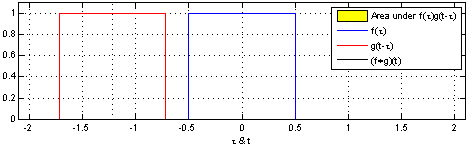
\includegraphics[scale=1.8]{../images/conv1.png}
\end{figure}
\begin{figure}[H]{}
    \centering
    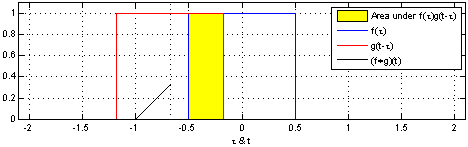
\includegraphics[scale=1.8]{../images/conv2.png}
\end{figure}
\begin{figure}[H]{}
    \centering
    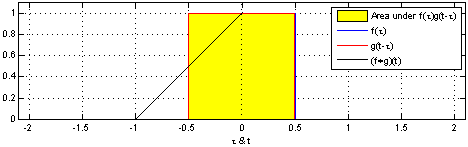
\includegraphics[scale=1.8]{../images/conv3.png}
\end{figure}
\begin{figure}[H]{}
    \centering
    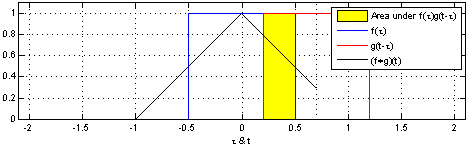
\includegraphics[scale=1.8]{../images/conv4.png}
\end{figure}
\begin{figure}[H]{}
    \centering
    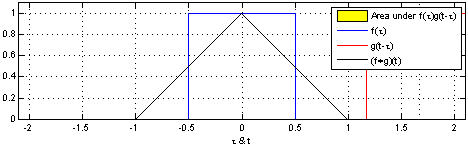
\includegraphics[scale=1.8]{../images/conv5.png}
\end{figure}

Le reti convoluzionali sfrutteranno questo tipo di 
operazione nel caso di immagini.\\ Mostriamo il seguente esempio:

\begin{figure}[H]{}
    \centering
    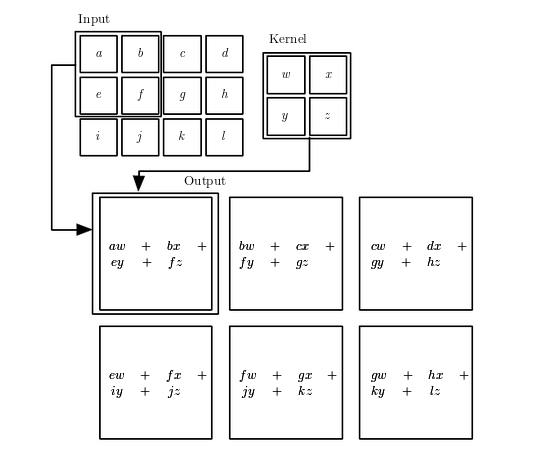
\includegraphics[scale=2.5]{../images/2conv.png}
    \captionof{figure}{esempio di convoluzione 2D}\label{fig:cc}
\end{figure}

%%%%%%%%%%%%%%%%%%%%%%%%%%%%%%%%%%%%%%%%%%%%%%%%%%%%%%%%%%%%%%%%%%%%%%%%%%%
%%%%%%%%%%%%%%%%%%%%%%%%%%%%%%%%%%%%%%%%%%%%%%%%%%%%%%%%%%%%%%%%%%%%%%%%%%%
%%%%%%%%%%%%%%%%%%%%%%%%%%%%%%%%%%%%%%%%%%%%%%%%%%%%%%%%%%%%%%%%%%%%%%%%%%%


\subsection{CNN: Convolutional Neural Network}

Sono delle reti neurali specializzate nel processamento
di dati che hanno una rappresentazione a griglia (come immagini).\\
Utilizzano layer convoluzionali che sfruttano kernel/finestre di
dimensione variabile che, scorrendo l'immagine, si attivano quando
riconoscono particolari caratteristiche.\\
L'introduzione dei layer convoluzionali migliora l'apprendimendo
soprattutto grazie a 3 caratteristiche:
\begin{enumerate}
    \item Interazioni sparse: l'utilizzo di kernel piccoli
    permette di avere un numero ridotto di pesi (parametri) da
    apprendere, rispetto ad un layer completamente connesso.
    Questo permette di avere un apprendimento essenzialmente
    più veloce.
    \item Condivisione dei parametri: gli stessi parametri di 
    un kernel vengono usati per riconoscere particolari feature
    all'interno dell'immagine in punti differenti.
    n.b. il kernel scorre su tutta l'immagine.
    \item Equivarianza rispetto a traslazioni: i medesimo
    kernel è in grado di riconoscere la medesima feature anche
    in punti differenti all'interno dell'immagine.
\end{enumerate}

Dopo aver applicato un layer convoluzionale viene utilizzata 
anche in questo caso una funzione di attivazione.\\
In ultimo si utilizza un layer di Pooling che ha il compito di
semplificare l'immagine. Un esempio comune è quello
di max pooling, in cui ogni ouput del layer precedente viene
aggiornato al valore massimo del suo vicinato.

\begin{figure}[H]{}
    \centering
    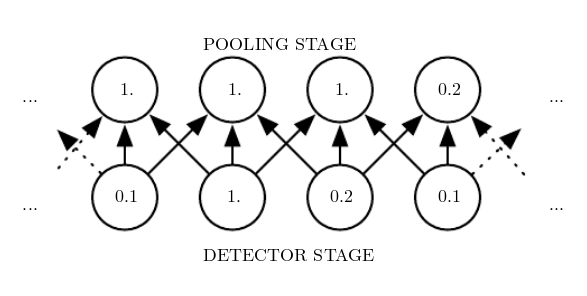
\includegraphics[scale=2.5]{../images/pooling.png}
    \captionof{figure}{Max Pooling}\label{fig:cc}
\end{figure}

Solitamente questi tre layer (convoluzione, attivazione, pooling)
possono essere denotati come singolo layer convoluzionale.

\begin{figure}[H]{}
    \centering
    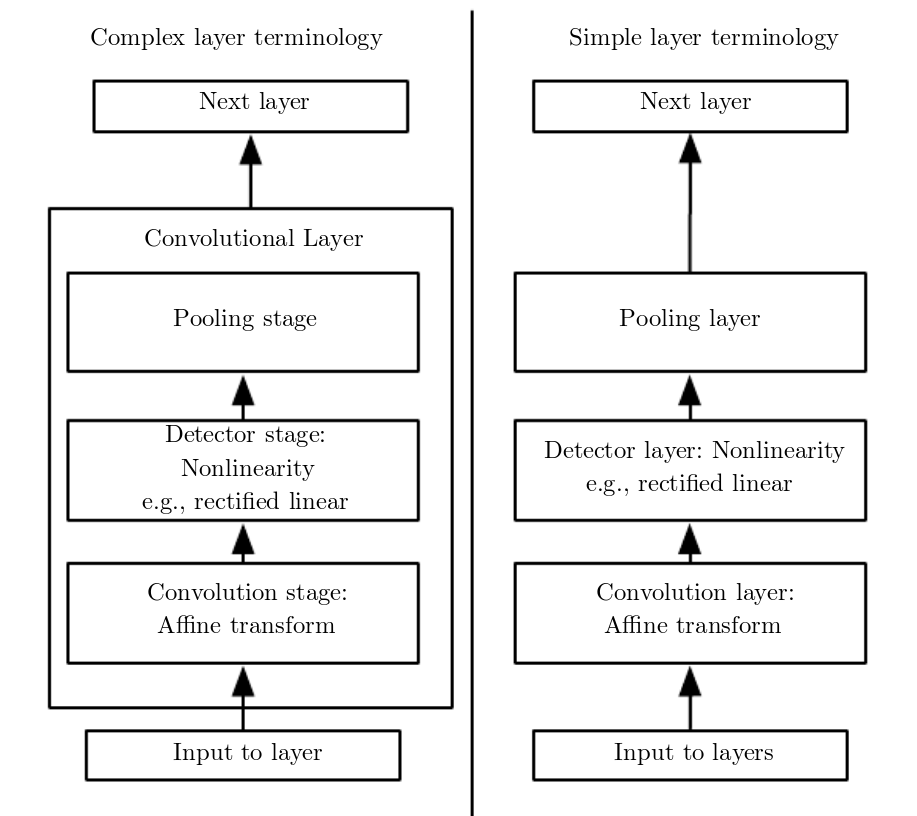
\includegraphics[scale=2]{../images/cl.png}
    \captionof{figure}{Convolutional Layer}\label{fig:cc}
\end{figure}

L'idea di fondo è quella di utilizzare i livelli convolutivi
per spezzare l'informazione contenuta nell'immaggine con lo
scopo di ottenere un vettore di feature che sia facile
da classificare direttamente con un MLPNN.
In ultimo illustriamo l'intero processo della rete neurale su un'immagine.

\begin{figure}[H]{}
    \centering
    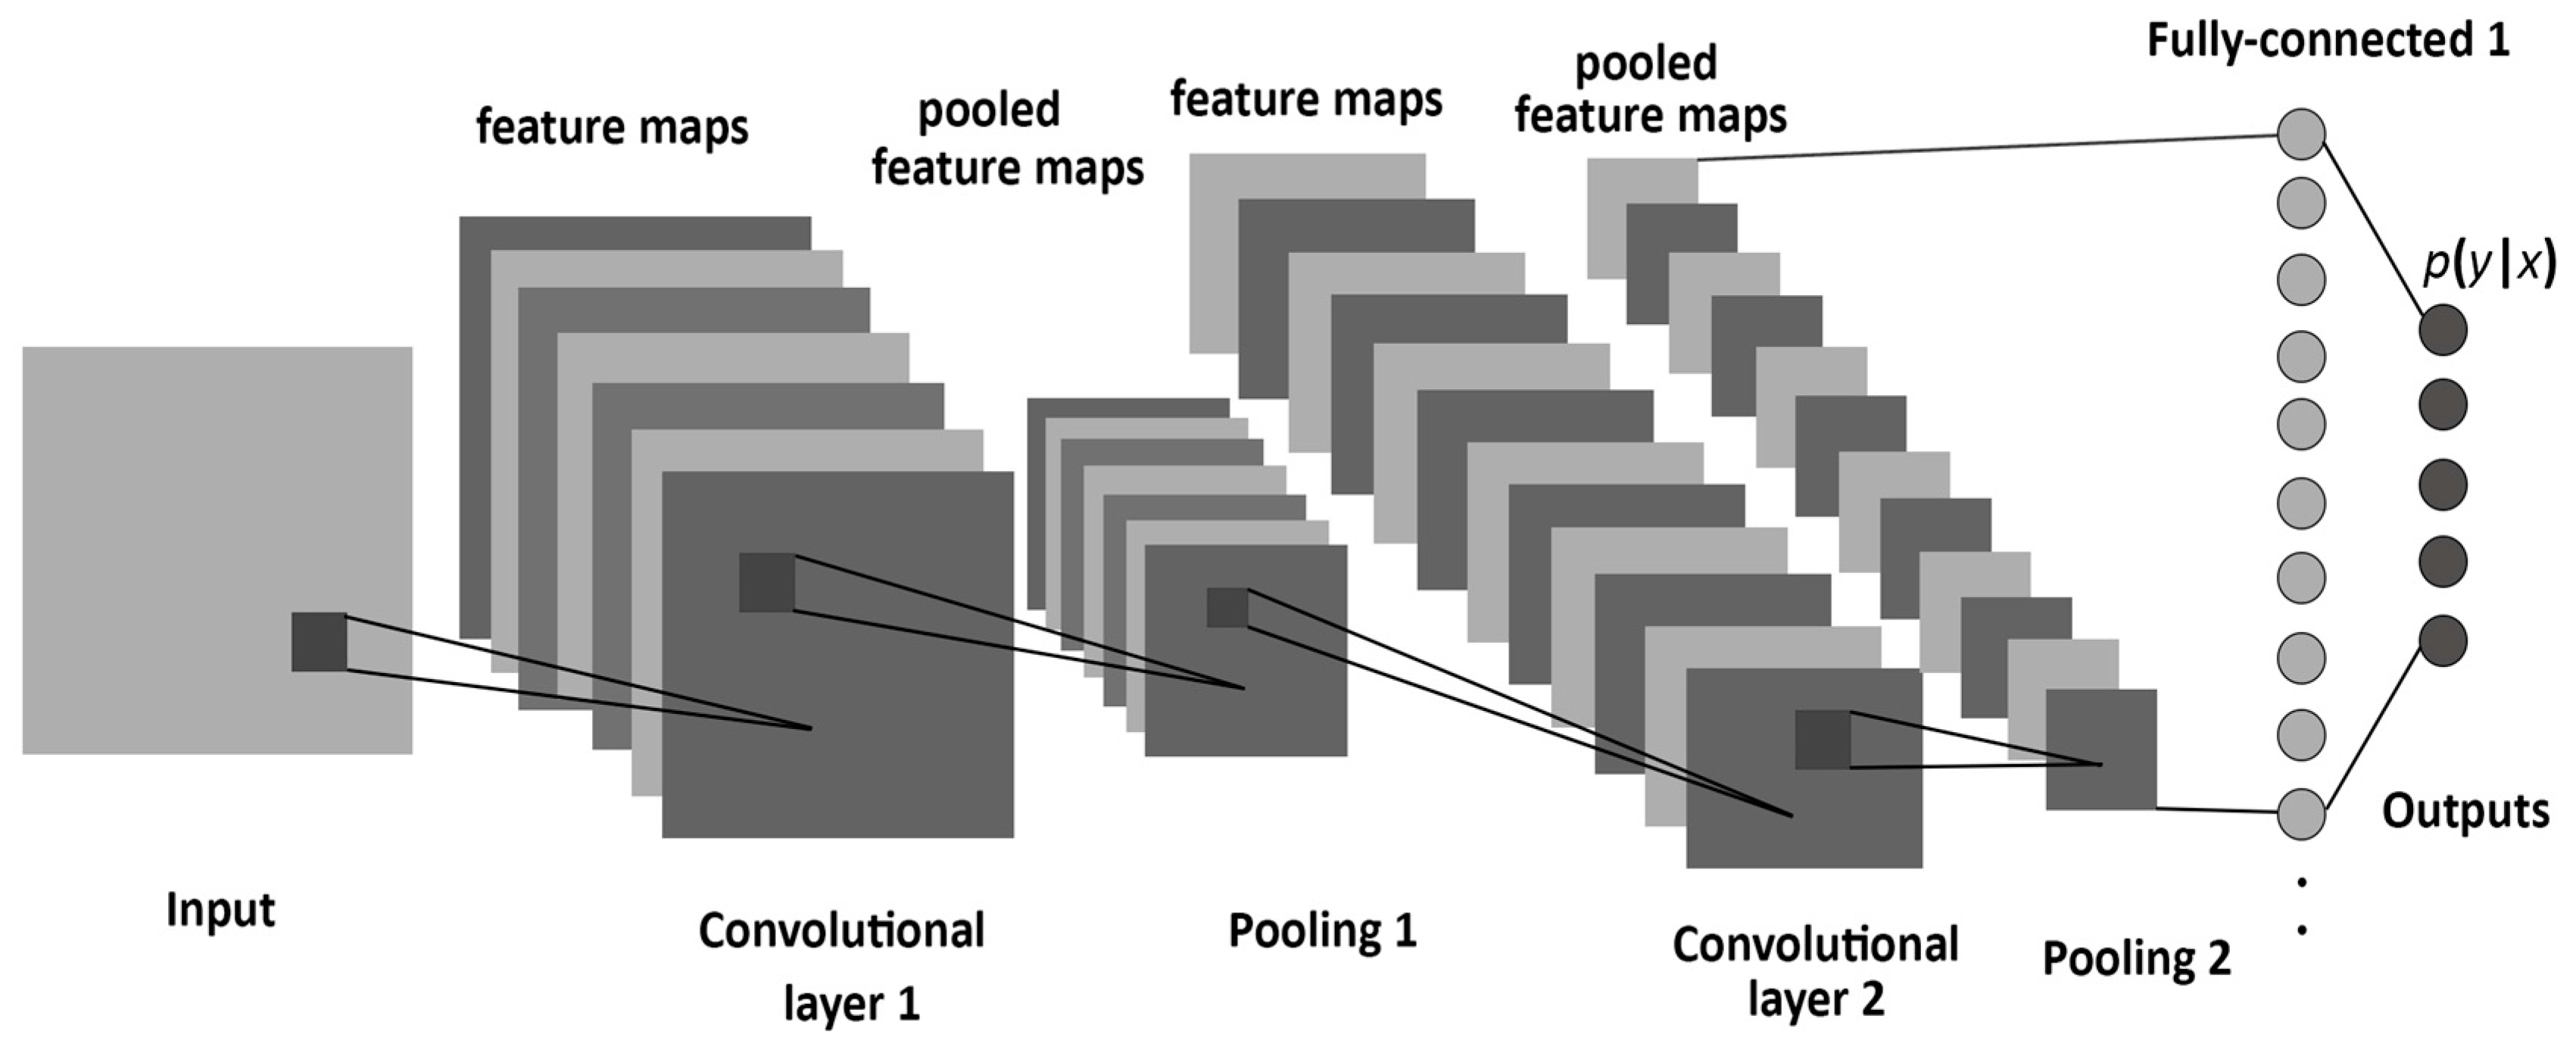
\includegraphics[scale=1]{../images/convex.png}
    \captionof{figure}{CNN su di una immagine}\label{fig:cc}
\end{figure}

%%%%%%%%%%%%%%%%%%%%%%%%%%%%%%%%%%%%%%%%%%%%%%%%%%%%%%%%%%%%%%%%%%%%%%%%%%%
%%%%%%%%%%%%%%%%%%%%%%%%%%%%%%%%%%%%%%%%%%%%%%%%%%%%%%%%%%%%%%%%%%%%%%%%%%%
%%%%%%%%%%%%%%%%%%%%%%%%%%%%%%%%%%%%%%%%%%%%%%%%%%%%%%%%%%%%%%%%%%%%%%%%%%%

\subsection{Dropout}

E' un concetto tanto semplice quanto efficace, applicato
esclusivamente in ambito di reti neurali.\\
Lo scopo è quello di prevenire l'everfitting.\\
Essenzialmente scegliamo in modo arbitrario una probabilità
tale per cui alcuni neuroni verrano tagliati fuori dal backward step
e da forward step durante la fase di apprendimento.\\
Questo forza la rete ad apprendere nuovi "percorsi" per attivare
un determinato neurone.

\begin{figure}[H]{}
    \centering
    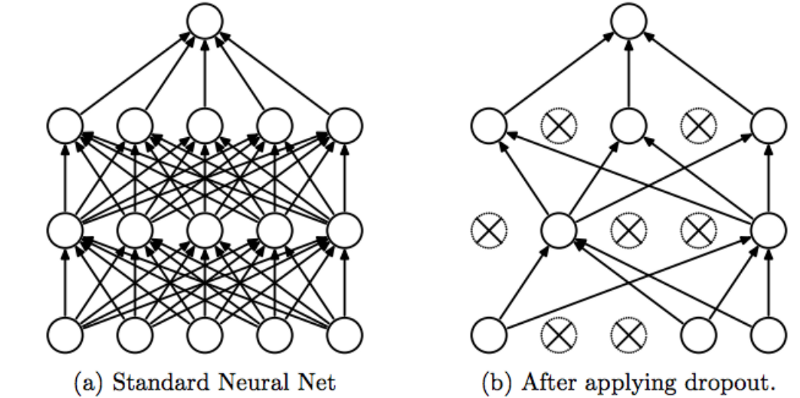
\includegraphics[scale=0.5]{../images/drop.png}
    \captionof{figure}{Esempio di Dropout}\label{fig:cc}
\end{figure}

Valori di Dropout troppo alti compromettono l'apprendimento, mentre
valori troppo bassi non beneficiano della mitigazione dell'overfitting.
In diverse prove un valore ragionevole, che non vanifica il training,
si è rivelato essere 0.2.

%%%%%%%%%%%%%%%%%%%%%%%%%%%%%%%%%%%%%%%%%%%%%%%%%%%%%%%%%%%%%%%%%%%%%%%%%%%
%%%%%%%%%%%%%%%%%%%%%%%%%%%%%%%%%%%%%%%%%%%%%%%%%%%%%%%%%%%%%%%%%%%%%%%%%%%
%%%%%%%%%%%%%%%%%%%%%%%%%%%%%%%%%%%%%%%%%%%%%%%%%%%%%%%%%%%%%%%%%%%%%%%%%%%

\subsection{RMSprop}

E' un metodo di ottimizazzione per la scelta del learning rate,
proposto da Geoff Hinton.\\
L'idea è quella di non seguire cecamente il gradiente
ad ogni passo, ma di seguire il gradiente nuovamente ottenuto,
pesato per un termine $\beta$ e sommato alla media di tutti i gradienti
ottenuti fino all'ultimo (in modo tale da ricordare il passato), anche questo
pesato per un termine $(1-\beta)$. Formalmente:
\begin{equation}E[\Delta^2]_t = \beta E[\Delta^2]_{t-1}+(1-\beta)\Delta^2_t\end{equation}
Solitamente viene indicato come valore di $\beta=0.9$.
A questo punto l'aggiornamento di ciascun peso sarà:
\begin{equation}
w_{t+1}=w_t-\frac{\alpha}{\sqrt{E[\Delta^2]_t+\epsilon}}\Delta_t
\end{equation}
Dove $\alpha$ rappresenta il learning rate comune.
Mentre $\frac{\alpha}{\sqrt{E[\Delta^2]_t}}$ rappresenta il termine
di regolarizzazione.

%%%%%%%%%%%%%%%%%%%%%%%%%%%%%%%%%%%%%%%%%%%%%%%%%%%%%%%%%%%%%%%%%%%%%%%%%%%
%%%%%%%%%%%%%%%%%%%%%%%%%%%%%%%%%%%%%%%%%%%%%%%%%%%%%%%%%%%%%%%%%%%%%%%%%%%
%%%%%%%%%%%%%%%%%%%%%%%%%%%%%%%%%%%%%%%%%%%%%%%%%%%%%%%%%%%%%%%%%%%%%%%%%%%


\section{Models}
Per costruire un riconoscitore efficace sono stati testati diversi modelli:
\begin{enumerate}
    \item MLPNN: Una rete a diversi livelli completamente conessa.
    \item CNN\cite{cnn}: Una rete convoluzionale che sfrutta kernel di dimensioni ridotte
               per la classificazione delle immagini.
    \item Committees: Comitati di esperti che prendono decisioni basate sulla maggioranza.
\end{enumerate}


%%%%%%%%%%%%%%%%%%%%%%%%%%%%%%%%%%%%%%%%%%%%%%%%%%%%%%%%%%%%%%%%%%%%%%%%%%%
%%%%%%%%%%%%%%%%%%%%%%%%%%%%%%%%%%%%%%%%%%%%%%%%%%%%%%%%%%%%%%%%%%%%%%%%%%%
%%%%%%%%%%%%%%%%%%%%%%%%%%%%%%%%%%%%%%%%%%%%%%%%%%%%%%%%%%%%%%%%%%%%%%%%%%%

\subsection{built MLPNN}

L'obbiettivo è quello di confrontare diverse architetture a parità
di Dropout, e funzioni di attivazione. 
Vogliamo verificare quanto la profondità della rete, la dimensione
di ciascun layer e il numero di parametri totali influenza le capacità di 
apprendimento.
 \newpage

\begin{multicols}{3}

    \noindent
    \begin{minipage}{\linewidth}
        \centering
        \includegraphics[width=5cm]{../mnist_models/MLPNN_type3-batch128-balanced/model.png}
        \captionof{figure}{Modello basso con layer ristretti.\\ Il miglior modello
        ottiene come accuracy e loss sul set di validazione i rispettivi risultati:
        0.972 e 0.107.}\label{fig:cc}
    \end{minipage}
    \bigskip

    \noindent
    \begin{minipage}{\linewidth}
        \centering
        \includegraphics[width=5cm]{../mnist_models/MLPNN_type2-batch128-balanced/model.png}
        \captionof{figure}{Modello basso con layer ampi.\\ Il miglior modello
        ottiene come accuracy e loss sul set di validazione i rispettivi risultati:
        0.982 e 0.067.}\label{fig:cc}
    \end{minipage}
    \bigskip

    \noindent
    \begin{minipage}{\linewidth}
        \centering
        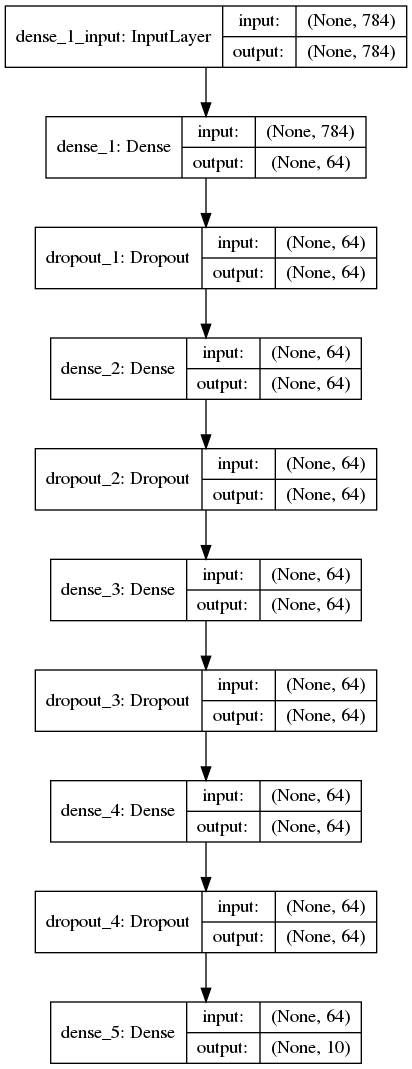
\includegraphics[width=5cm]{../mnist_models/MLPNN_type1-batch128-balanced/model.png}
        \captionof{figure}{Modello profondo con layer ristretti.\\ Il miglior modello
        ottiene come accuracy e loss sul set di validazione i rispettivi risultati:
        0.970 e 0.123.}\label{fig:cc}
    \end{minipage}
    \bigskip


    \noindent
    \begin{minipage}{\linewidth}
        \centering
        \includegraphics[width=5cm]{../mnist_models/MLPNN_type4-batch128-balanced/model.png}
        \captionof{figure}{Modello basso con layer ampi.\\ Il miglior modello
        ottiene come accuracy e loss sul set di validazione i rispettivi risultati:
        0.980 e 0.115.}\label{fig:cc}
    \end{minipage}
    \bigskip

\end{multicols}
Per ciascuno dei modelli sono stati eseguite 100 epoche di apprendimento
con tecnica mini-batch di dimensione 128.\\


Premettendo che tutti i modelli hanno un ottimo comportamento, l'unico 
che spicca veramente è un quello mostrato in figura 11, con un singolo
layer nascosto e una archittura "ampia".\\

Rispettivamente le reti profonde non ottengono dei risultati altrettanto buoni,
questo dimostra che le capacità di generalizzazione di una rete si possono
sviluppare anche in ampiezza.

Consideriamo ora l'andamento della loss e della accuracy per tutti e quattro i modelli.\\
Prima i Modelli non profondi:

\begin{multicols}{2}
    \noindent
    \begin{minipage}{\linewidth}
        \centering
        \includegraphics[width=9cm]{../mnist_models/MLPNN_type3-batch128-balanced/0test_loss_acc.png}
        \captionof{figure}{Loss del modello basso con layer ristretti.}\label{fig:cc}
    \end{minipage}
    \bigskip

    \noindent
    \begin{minipage}{\linewidth}
        \centering
        \includegraphics[width=9cm]{../mnist_models/MLPNN_type3-batch128-balanced/0train_loss_acc.png}
        \captionof{figure}{Accuracy del modello basso con layer ristretti.}\label{fig:cc}
    \end{minipage}
    \bigskip
\end{multicols}

\begin{multicols}{2}
    \noindent
    \begin{minipage}{\linewidth}
        \centering
        \includegraphics[width=9cm]{../mnist_models/MLPNN_type2-batch128-balanced/0test_loss_acc.png}
        \captionof{figure}{Loss del modello basso con layer ampi.}\label{fig:cc}
    \end{minipage}
    \bigskip

    \noindent
    \begin{minipage}{\linewidth}
        \centering
        \includegraphics[width=9cm]{../mnist_models/MLPNN_type2-batch128-balanced/0train_loss_acc.png}
        \captionof{figure}{Accuracy del modello basso con layer ampi.}\label{fig:cc}
    \end{minipage}
    \bigskip
\end{multicols}

Come si può notare facilmente dalle figure, e sarà confermato anche in seguito,
modelli ampi ottengono risultati migliori in tempi minori.\\
Infatti il modello ottimo viene ottenuto già entro le prime 20 epoche
di addestramento, per quanto riguarda architetture ampie.\\

Vediamo ora l'andamento per le architetture profonde.

\begin{multicols}{2}
    \noindent
    \begin{minipage}{\linewidth}
        \centering
        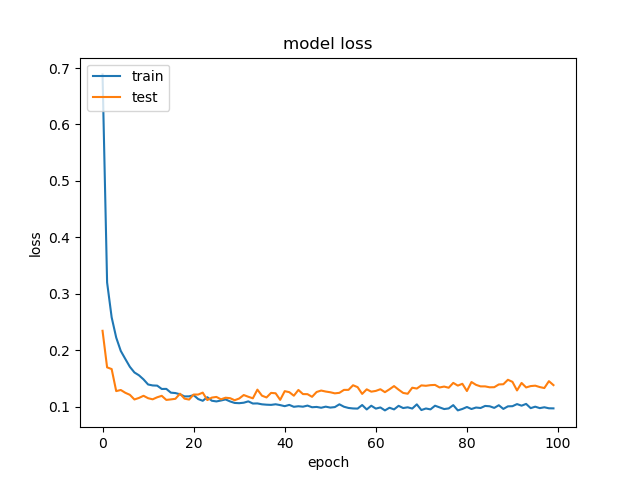
\includegraphics[width=9cm]{../mnist_models/MLPNN_type1-batch128-balanced/0test_loss_acc.png}
        \captionof{figure}{Loss del modello profondo con layer ristretti.}\label{fig:cc}
    \end{minipage}
    \bigskip

    \noindent
    \begin{minipage}{\linewidth}
        \centering
        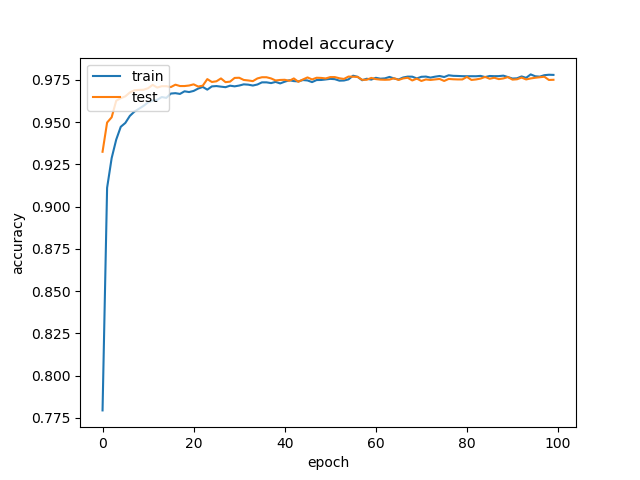
\includegraphics[width=9cm]{../mnist_models/MLPNN_type1-batch128-balanced/0train_loss_acc.png}
        \captionof{figure}{Accuracy del modello profondo con layer ristretti.}\label{fig:cc}
    \end{minipage}
    \bigskip
\end{multicols}

\begin{multicols}{2}
    \noindent
    \begin{minipage}{\linewidth}
        \centering
        \includegraphics[width=9cm]{../mnist_models/MLPNN_type4-batch128-balanced/0test_loss_acc.png}
        \captionof{figure}{Loss del modello profondo con layer ampi.}\label{fig:cc}
    \end{minipage}
    \bigskip

    \noindent
    \begin{minipage}{\linewidth}
        \centering
        \includegraphics[width=9cm]{../mnist_models/MLPNN_type4-batch128-balanced/0train_loss_acc.png}
        \captionof{figure}{Accuracy del modello profondo con layer ampi.}\label{fig:cc}
    \end{minipage}
    \bigskip
\end{multicols}

Riconfermiamo quindi ciò che è stato già detto: layer ampi favoriscono
la velocità di apprendimento in termini di epoche (chiaramente ciascuna
epoca ha una durata più lunga, dato il numero maggiore di parametri
da aggiornare).

%%%%%%%%%%%%%%%%%%%%%%%%%%%%%%%%%%%%%%%%%%%%%%%%%%%%%%%%%%%%%%%%%%%%%%%%%%%
%%%%%%%%%%%%%%%%%%%%%%%%%%%%%%%%%%%%%%%%%%%%%%%%%%%%%%%%%%%%%%%%%%%%%%%%%%%
%%%%%%%%%%%%%%%%%%%%%%%%%%%%%%%%%%%%%%%%%%%%%%%%%%%%%%%%%%%%%%%%%%%%%%%%%%%

\newpage
\subsection{built CNN}

Questa volta lo scopo è quello di valutare come varia l'apprendimento
in funzione della dimensione dei kernel e in funzione della
dimensionalità dei layer convoluzionali.\\

Vediamo quindi l'architettura di ciascun modello:

\begin{multicols}{3}

    \noindent
    \begin{minipage}{\linewidth}
        \centering
        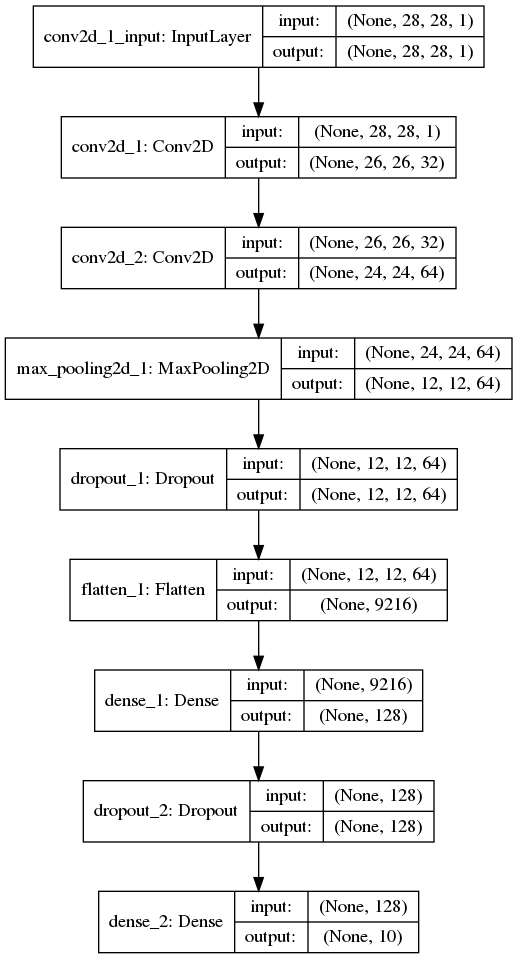
\includegraphics[width=5cm]{../mnist_models/CNN2D_type0-batch128-balanced/model.png}
        \captionof{figure}{Modello con kernel e layer ridotti.\\ Il miglior modello
        ottiene come accuracy e loss sul set di validazione i rispettivi risultati:
        0.993 e 0.025.}\label{fig:cc}
    \end{minipage}
    \bigskip

    \noindent
    \begin{minipage}{\linewidth}
        \centering
        \includegraphics[width=5cm]{../mnist_models/CNN2D_type1-batch128-balanced/model.png}
        \captionof{figure}{Modello con kernel ampi e layer ridotti.\\ Il miglior modello
        ottiene come accuracy e loss sul set di validazione i rispettivi risultati:
        0.991 e 0.037.}\label{fig:cc}
    \end{minipage}
    \bigskip

    \noindent
    \begin{minipage}{\linewidth}
        \centering
        \includegraphics[width=5cm]{../mnist_models/CNN2D_type2-batch128-balanced/model.png}
        \captionof{figure}{Modello con kernel ristretti e layer ampi.\\ Il miglior modello
        ottiene come accuracy e loss sul set di validazione i rispettivi risultati:
        0.987 e 0.051.}\label{fig:cc}
    \end{minipage}
    \bigskip

    \noindent
    \begin{minipage}{\linewidth}
        \centering
        \includegraphics[width=5cm]{../mnist_models/CNN2D_type3-batch128-balanced/model.png}
        \captionof{figure}{Modello con kernel e layer ampi.\\ Il miglior modello
        ottiene come accuracy e loss sul set di validazione i rispettivi risultati:
        0.989 e 0.050.}\label{fig:cc}
    \end{minipage}
    \bigskip

\end{multicols}

Il modello che ottiene i risultati migliori dunque è quello che viene mostrato
in figura 22. In questo caso la rete utilizza kernel $3\times3$ con layer di dimensione 64.\\

Tuttavia ancora una volta i risultati delle architetture alternative sono estremamente
positivi tanto da risultare praticamente equivalenti.\\

Apparentemente in questo contesto la scelta di un kernel grande o piccolo
non va ad influenzare l'apprendimento. Lo stesso vale per la dimensionalità
dei layer.\\

Ciò che comunque risulta evidente fin da subito è che le reti convoluzionali
hanno un impatto decisamente migliore rispetto ai percettroni multistrato,
ottenedo degli score estremamente più positivi.\\

Andiamo ancora una volta a valutare l'andamento dell'apprendimento nei
termini di loss e accuracy delle diversi reti.

\begin{multicols}{2}
    \noindent
    \begin{minipage}{\linewidth}
        \centering
        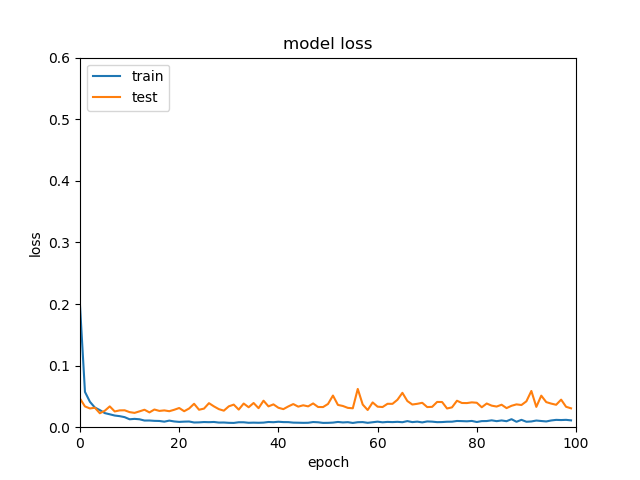
\includegraphics[width=9cm]{../mnist_models/CNN2D_type0-batch128-balanced/0test_loss_acc.png}
        \captionof{figure}{Loss del modello con kernel e layer ridotti.}\label{fig:cc}
    \end{minipage}
    \bigskip

    \noindent
    \begin{minipage}{\linewidth}
        \centering
        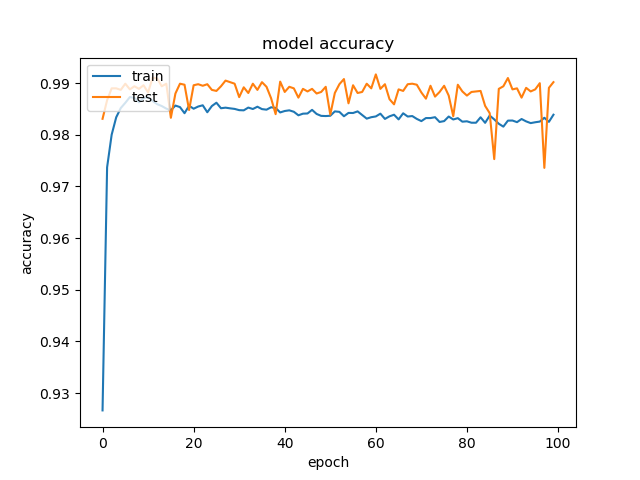
\includegraphics[width=9cm]{../mnist_models/CNN2D_type0-batch128-balanced/0train_loss_acc.png}
        \captionof{figure}{Accuracy del modello con kernel e layer ridotti.}\label{fig:cc}
    \end{minipage}
    \bigskip
\end{multicols}

\begin{multicols}{2}
    \noindent
    \begin{minipage}{\linewidth}
        \centering
        \includegraphics[width=9cm]{../mnist_models/CNN2D_type1-batch128-balanced/0test_loss_acc.png}
        \captionof{figure}{Loss del modello con kernel ampi e layer ridotti.}\label{fig:cc}
    \end{minipage}
    \bigskip

    \noindent
    \begin{minipage}{\linewidth}
        \centering
        \includegraphics[width=9cm]{../mnist_models/CNN2D_type1-batch128-balanced/0train_loss_acc.png}
        \captionof{figure}{Accuracy del modello con kernel ampi e layer ridotti.}\label{fig:cc}
    \end{minipage}
    \bigskip
\end{multicols}

L'unica differenza tra figure 26-27 e 28-29 è la dimensionalità dei kernel, che, nel
secondo caso sono più ampi. Ancora una volta possiamo riconfermare che la variazione
in dimensione non porta a cambiamenti significativi.\\


Mostriamo anche le ultime 4 figure:\newpage

\begin{multicols}{2}
    \noindent
    \begin{minipage}{\linewidth}
        \centering
        \includegraphics[width=9cm]{../mnist_models/CNN2D_type2-batch128-balanced/0test_loss_acc.png}
        \captionof{figure}{Loss del modello con kernel ampi e layer ristretti.}\label{fig:cc}
    \end{minipage}
    \bigskip

    \noindent
    \begin{minipage}{\linewidth}
        \centering
        \includegraphics[width=9cm]{../mnist_models/CNN2D_type2-batch128-balanced/0train_loss_acc.png}
        \captionof{figure}{Accuracy del modello con kernel ampi e layer ristretti.}\label{fig:cc}
    \end{minipage}
    \bigskip
\end{multicols}

\begin{multicols}{2}
    \noindent
    \begin{minipage}{\linewidth}
        \centering
        \includegraphics[width=9cm]{../mnist_models/CNN2D_type3-batch128-balanced/0test_loss_acc.png}
        \captionof{figure}{Loss del Modello con kernel e layer ampi.}\label{fig:cc}
    \end{minipage}
    \bigskip

    \noindent
    \begin{minipage}{\linewidth}
        \centering
        \includegraphics[width=9cm]{../mnist_models/CNN2D_type3-batch128-balanced/0train_loss_acc.png}
        \captionof{figure}{Accuracy del Modello con kernel e layer ampi.}\label{fig:cc}
    \end{minipage}
    \bigskip
\end{multicols}


Questa volta la differenza tra le figure 30-31 e 32-33 sta nell'ampiezza dei layer,
tuttavia, anche paragonando con le precedenti figure 26-27-28-29, non si riescono
a vedere delle differenze significative.

%%%%%%%%%%%%%%%%%%%%%%%%%%%%%%%%%%%%%%%%%%%%%%%%%%%%%%%%%%%%%%%%%%%%%%%%%%%
%%%%%%%%%%%%%%%%%%%%%%%%%%%%%%%%%%%%%%%%%%%%%%%%%%%%%%%%%%%%%%%%%%%%%%%%%%%
%%%%%%%%%%%%%%%%%%%%%%%%%%%%%%%%%%%%%%%%%%%%%%%%%%%%%%%%%%%%%%%%%%%%%%%%%%%


\section{Conclusions}

Diamo ora le ultime conclusione, anche alla luce del funzionamento
del riconoscitore.

%%%%%%%%%%%%%%%%%%%%%%%%%%%%%%%%%%%%%%%%%%%%%%%%%%%%%%%%%%%%%%%%%%%%%%%%%%%
%%%%%%%%%%%%%%%%%%%%%%%%%%%%%%%%%%%%%%%%%%%%%%%%%%%%%%%%%%%%%%%%%%%%%%%%%%%
%%%%%%%%%%%%%%%%%%%%%%%%%%%%%%%%%%%%%%%%%%%%%%%%%%%%%%%%%%%%%%%%%%%%%%%%%%%

\subsection{Examples}

\begin{figure}[H]{}
    \centering
    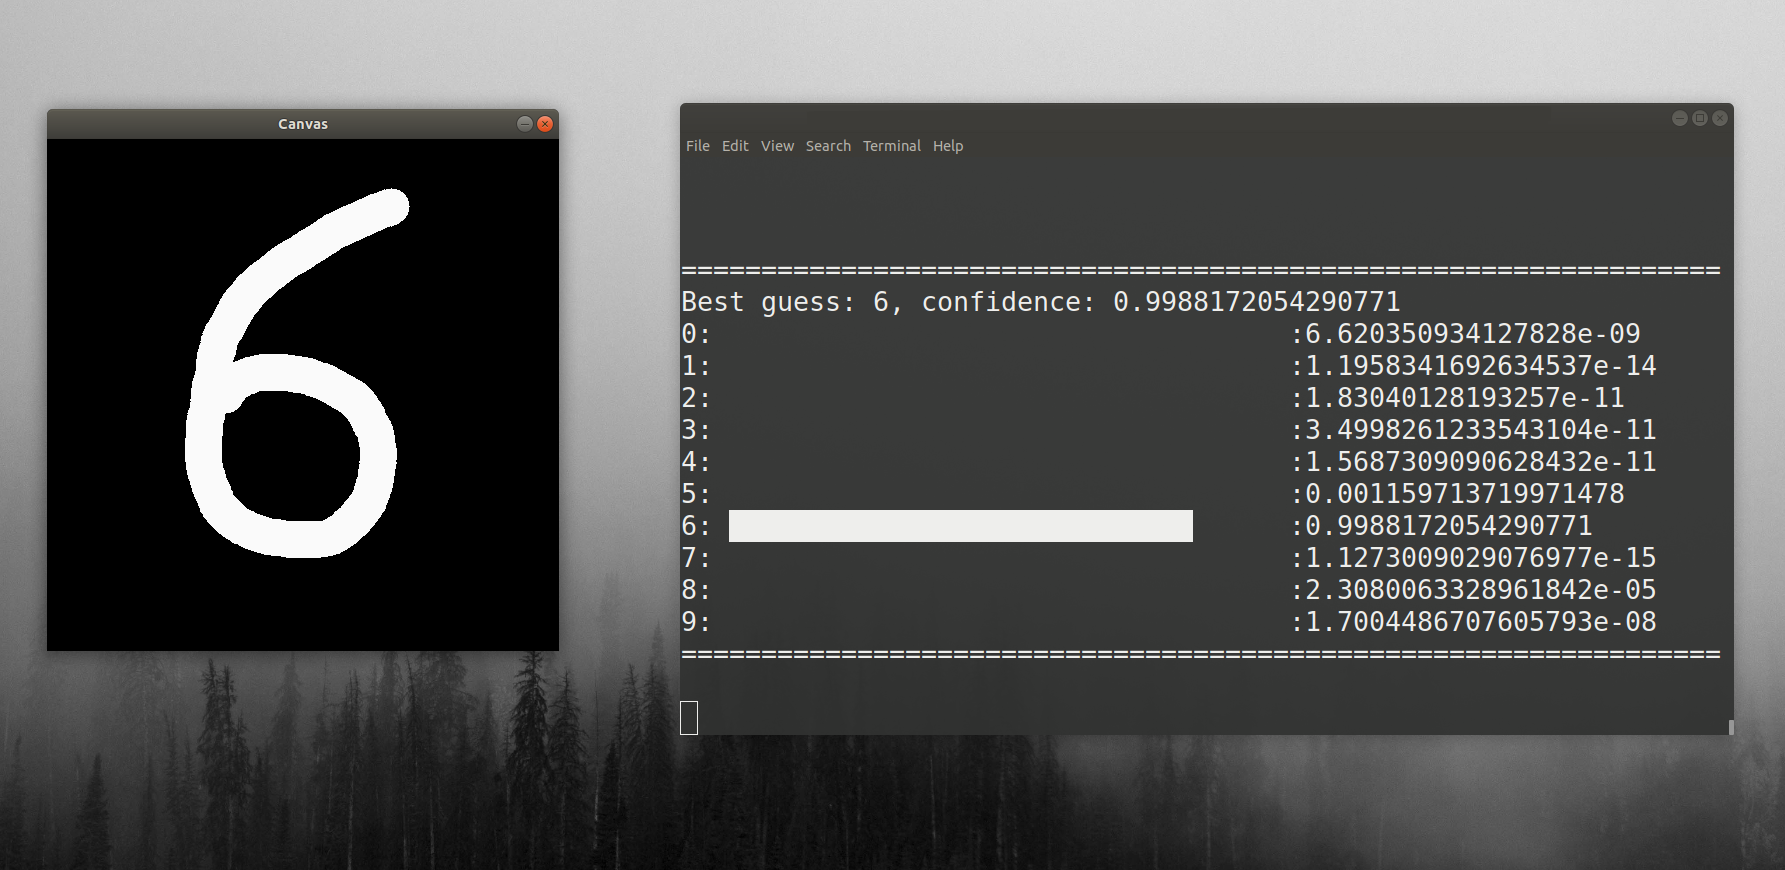
\includegraphics[scale=1]{../images/6ok.png}
    \captionof{figure}{6 riconosciuto come tale.}\label{fig:cc}
\end{figure}

\begin{figure}[H]{}
    \centering
    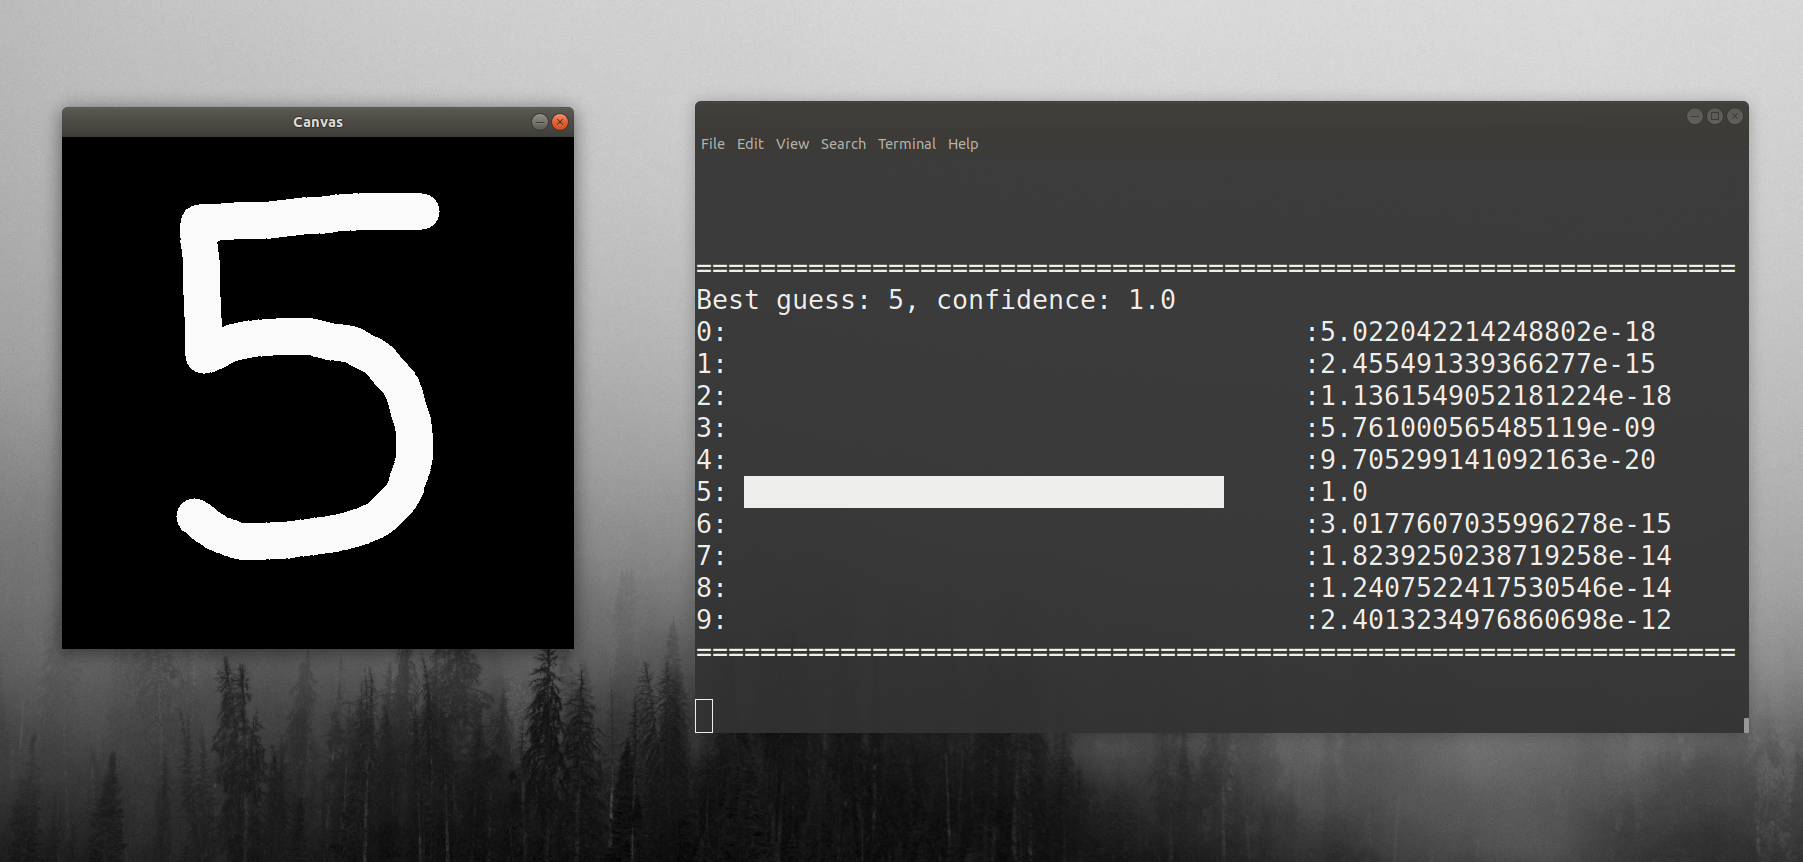
\includegraphics[scale=1]{../images/5ok.png}
    \captionof{figure}{5 riconosciuto come tale.}\label{fig:cc}
\end{figure}

Le precedenti cifre sono state disegnate in modo chiaro, e infatti
il riconoscitore funziona in modo corretto.\\

Mostriamo ora un caso limite:

\begin{figure}[H]{}
    \centering
    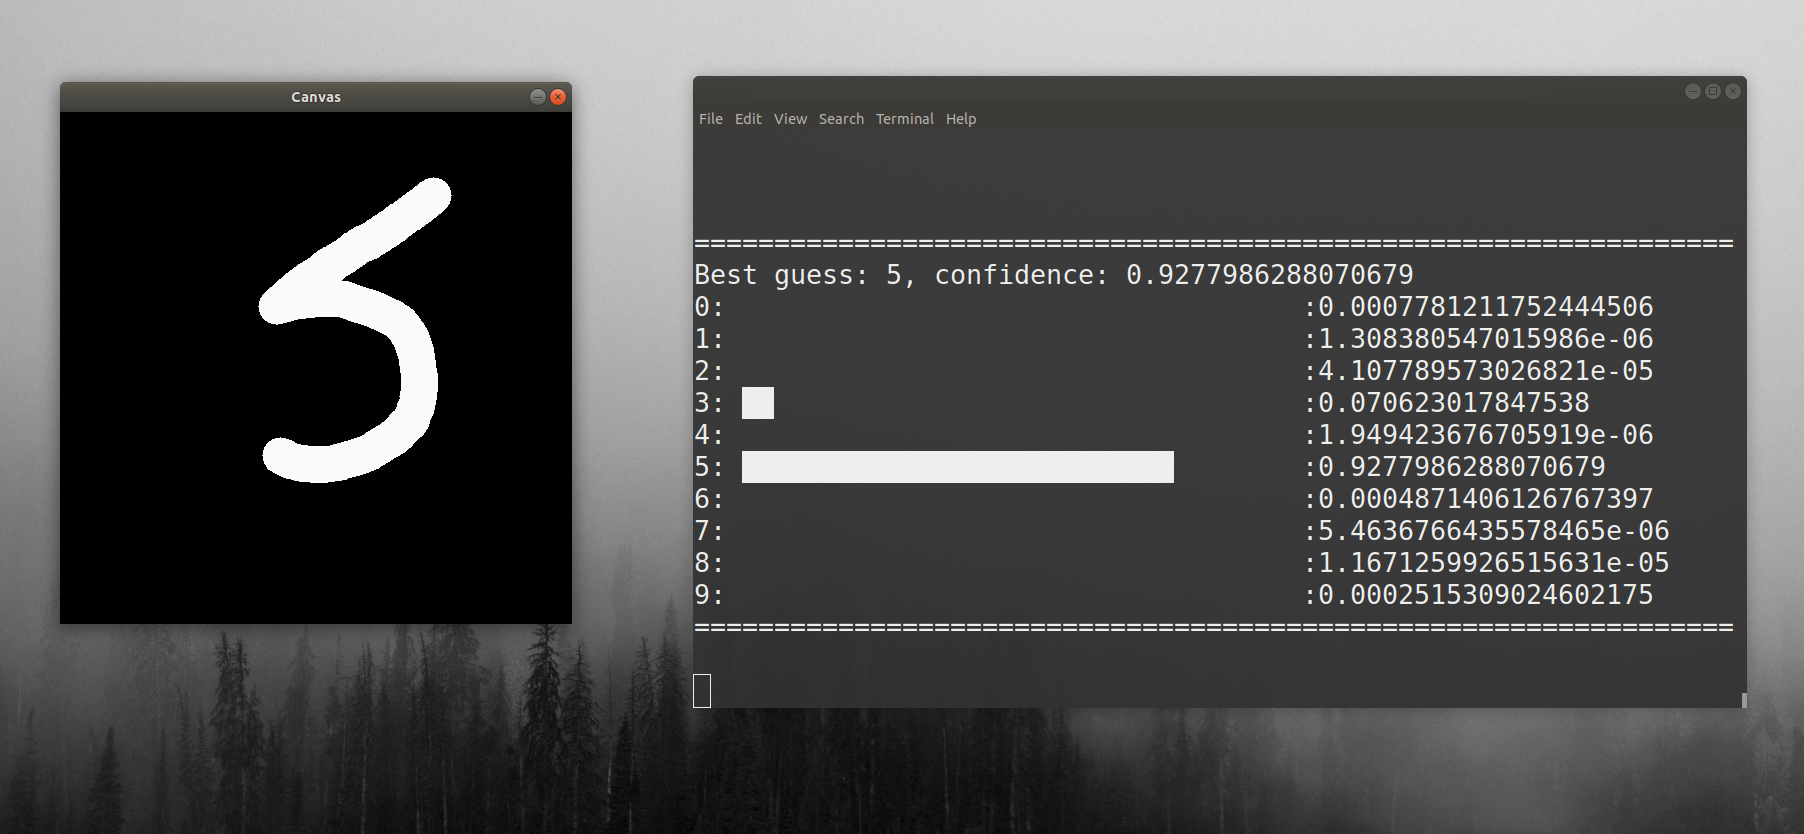
\includegraphics[scale=1]{../images/5meh.png}
    \captionof{figure}{5 limite riconosciuto come tale.}\label{fig:cc}
\end{figure}

Apparente è abbastanze comune all'interno del dataset mnist
la precedente versione del 5, questo porta a qualche confusione
soprattutto nei confronti del 6.

\begin{figure}[H]{}
    \centering
    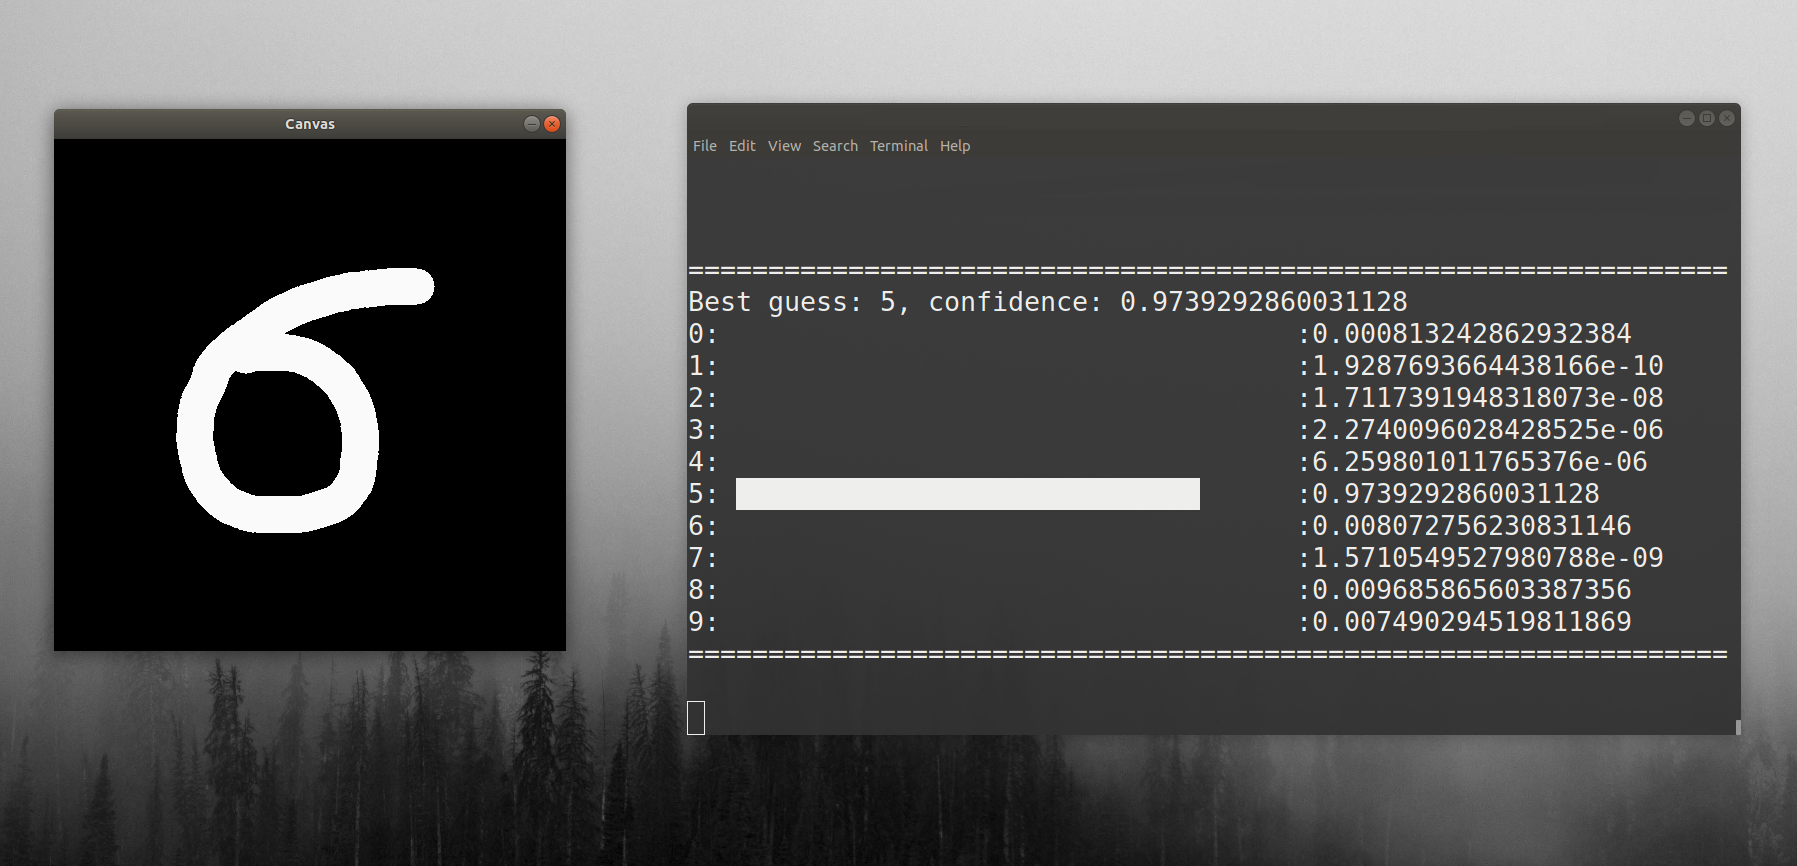
\includegraphics[scale=1]{../images/6no.png}
    \captionof{figure}{6 riconosciuto come 5.}\label{fig:cc}
\end{figure}

Lo stesso avviene anche per il 7 e l'1 che sono intrisecamente simili.

\begin{figure}[H]{}
    \centering
    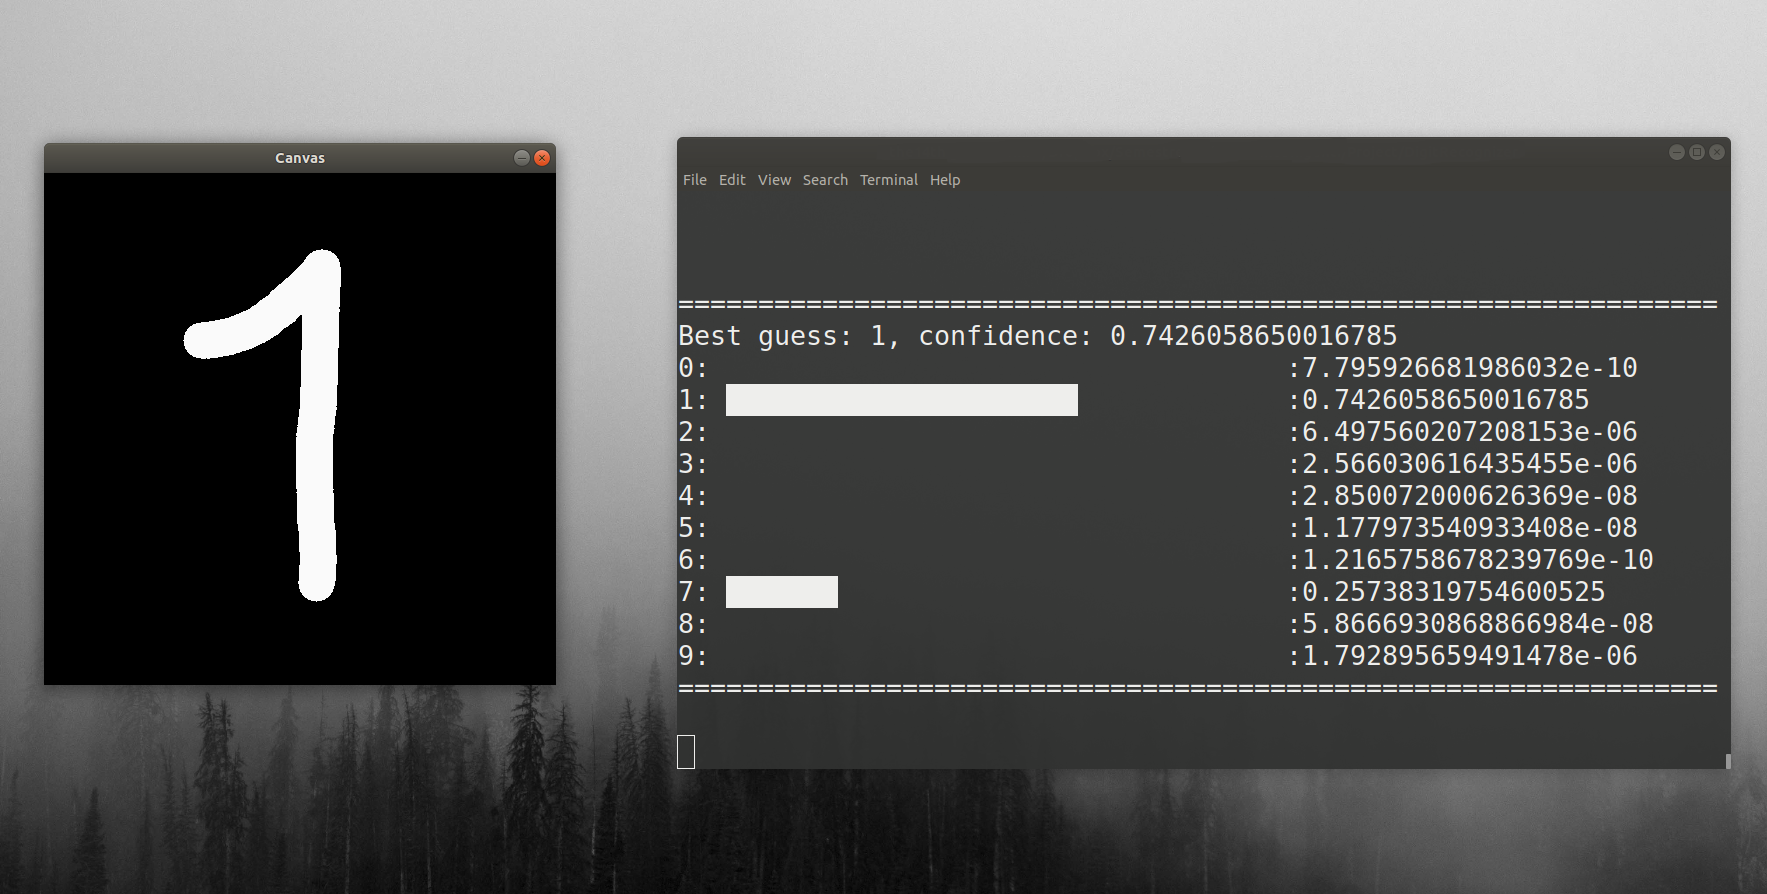
\includegraphics[scale=1]{../images/1meh.png}
    \captionof{figure}{1 riconosciuto come tale.}\label{fig:cc}
\end{figure}

Ma in questo caso, anche un operatore umano potrebbe avere qualche dubbio.

%%%%%%%%%%%%%%%%%%%%%%%%%%%%%%%%%%%%%%%%%%%%%%%%%%%%%%%%%%%%%%%%%%%%%%%%%%%
%%%%%%%%%%%%%%%%%%%%%%%%%%%%%%%%%%%%%%%%%%%%%%%%%%%%%%%%%%%%%%%%%%%%%%%%%%%
%%%%%%%%%%%%%%%%%%%%%%%%%%%%%%%%%%%%%%%%%%%%%%%%%%%%%%%%%%%%%%%%%%%%%%%%%%%

\subsection{Improvements}

Il riconoscitore funziona complessivamente bene, anche se in certi casi
commette errori.\\

Sicuramente è possibile avere un riconoscitore più preciso andando
ad ampliare il dataset con casi più diversificati e più numerosi, 
o eventualmente, facendo un oversampling delle immagini più critiche.\\

Un altra fonte di problemi sta nel fatto che le immagine del dataset sono
state scritte a mano su carta e digitalizzate in seguito.
Mentre quelle disegnate sulla finestra sono già digitali e vengono
semplicemente ridotte in dimensione fino a $28\times28$, in modo da essere
compatibili con le immagini nel mnist.\\
Nonostante la somiglianza comune, le nuove immagini non sono prodotte
nello stesso modo e questo può essere una causa contributiva alla misclassificazione
di alcuni esempi.



\subsection{References}

\begin{thebibliography}{9}


\bibitem{bengio}
    Goodfellow-et-al-2016,
    title={Deep Learning},
    author={Ian Goodfellow and Yoshua Bengio and Aaron Courville},
    publisher={MIT Press},
    note={http://www.deeplearningbook.org},
    year={2016}

\bibitem{gradient}
  Claude Lemarcéchal,\\
  \textit{https://www.math.uni-bielefeld.de/documenta/vol-ismp/40\_lemarechal-claude.pdf},
  2010.

\bibitem{rmsprop}
   Geoffrey E. Hinton,\\
  \textit{http://www.cs.toronto.edu/~tijmen/csc321/slides/lecture\_slides\_lec6.pdf}.

\bibitem{cnn}
   Alex Krizhevsky, Ilya Sutskever, Geoffrey E. Hinton, 
   ImageNet Classification with Deep Convolutional Neural Networks,
  \textit{https://papers.nips.cc/paper/4824-imagenet-classification-with-deep-convolutional-neural-networks.pdf}.

\bibitem{keras}
   \textit{https://github.com/keras-team/keras}

\bibitem{tensorflow}
   \textit{https://www.tensorflow.org/}

\bibitem{opencv}
   \textit{https://opencv.org/}


\end{thebibliography}

\end{document}
